\section{Support Vector Machines}

\subsection{Characteristics}
\begin{itemize}
    \item Supervised learning algorithm usually used for classification
    \item Binary classifier, so it is not probabilistic
    \item Linear classifier, but can perform nonlinear classification using particular kernels;
    \item Use regularized logistic regression
\end{itemize}

\subsection{Relation between Logistic Regression and SVM}
Logistic classification has the following formula:

\begin{equation} \tag*{}
    h_\theta(x) = g(\theta^Tx) = \cfrac{1}{1+e^{\theta^Tx}}
\end{equation}
Where:
\begin{equation} \tag*{}
    g(z) = \cfrac{1}{1+e^{-z}}
\end{equation}
The cost function for logistic regression given an example $i$ and a vector of weights $\theta$ is as follows:
\begin{equation} \tag*{}
    \text{cost} = -y^i \cdot \log(\frac{1}{1+e^{\theta^Tx^i}}) - (1-y^i) \cdot \log(1-\frac{1}{1+e^{\theta^Tx^i}})
\end{equation}
What we'd like logistic regression to do:
\begin{itemize}
    \item if $y = 1$, we want $h_\theta(x) \approx 1, \theta^Tx \gg 0$
    \item if $y = 0$, we want $h_\theta(x) \approx 0, \theta^Tx \ll 0$
\end{itemize}
\begin{center}
    \begin{tabular}{c}
        \\ 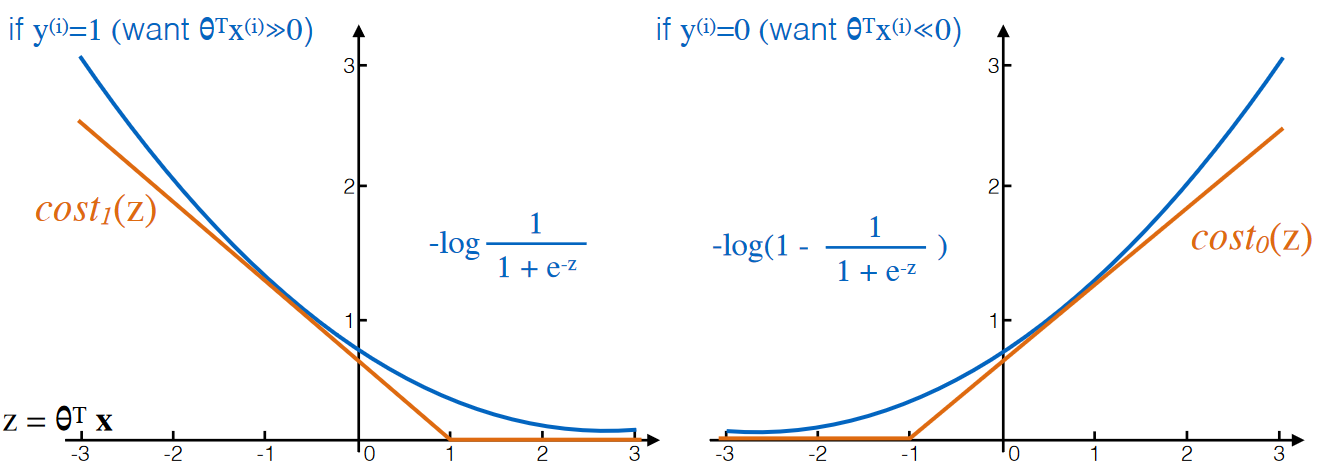
\includegraphics[width=0.9\textwidth]{images/SVM1.png} \\ \\
    \end{tabular}
\end{center}
The objective function of an SVM can be written as follows:
\begin{equation} \tag*{}
    \min \frac{1}{\lambda} \sum^m_{i=1} [y^i \cdot \text{cost}_1(\theta^Tx^i) + (1 - y^i) \cdot \text{cost}_0(\theta^Tx^i)] + \frac{1}{2} \sum^n_{j=i}\theta^2_j
\end{equation}
The functions cost$_1$ and cost$_0$ allow us to create a decision boundary.

\newpage